% !TeX spellcheck = en_GB
% \begin{figure}[t]
% 	\centering
% 	\begin{subfigure}[b]{0.49\textwidth}
% 		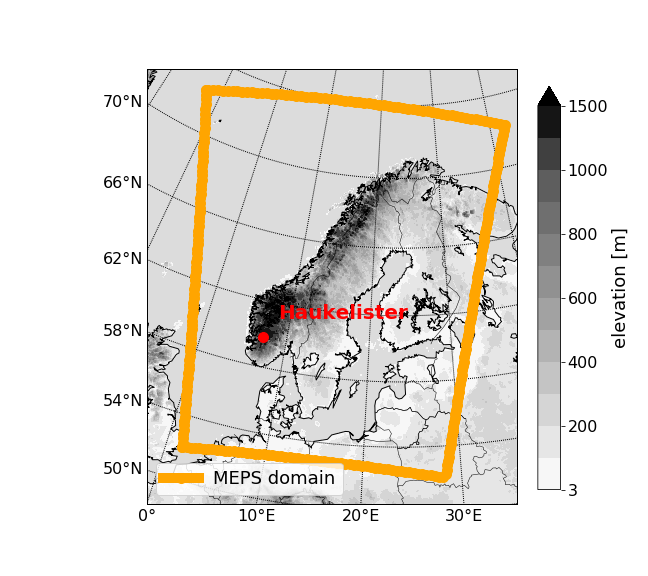
\includegraphics[trim={5.cm 1.8cm 5.8cm 2.3cm},clip,
% 		width=\textwidth]{./fig_Norway/Norway_MEPS}
% 		\caption{}\label{fig:site:Norway}
% 	\end{subfigure}
% 	%%%%% zoomed in map
% 	\begin{subfigure}[b]{0.49\textwidth}
% 		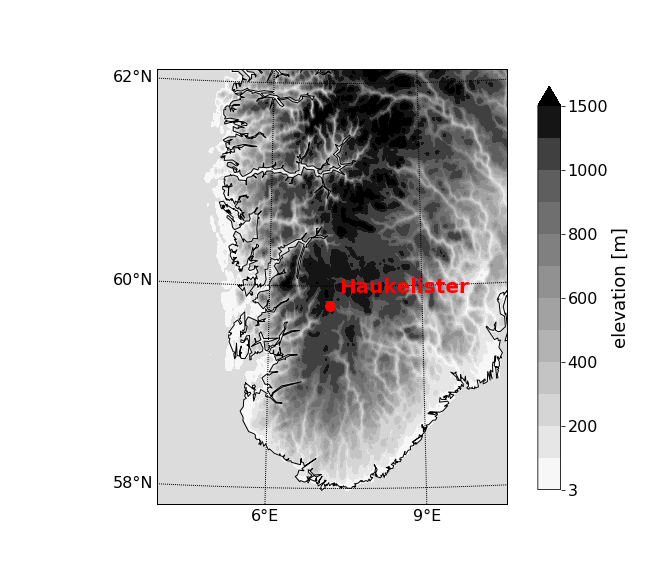
\includegraphics[trim={2.cm 1.8cm .65cm 2.3cm},clip,
% 		width=\textwidth]{./fig_Norway/South_Norway}
% 		\caption{}\label{fig:site:Nzoom}
% 	\end{subfigure}
% 	%%%%% zoomed in kartverketmap
% 	\begin{subfigure}[b]{0.32\textwidth}
% 		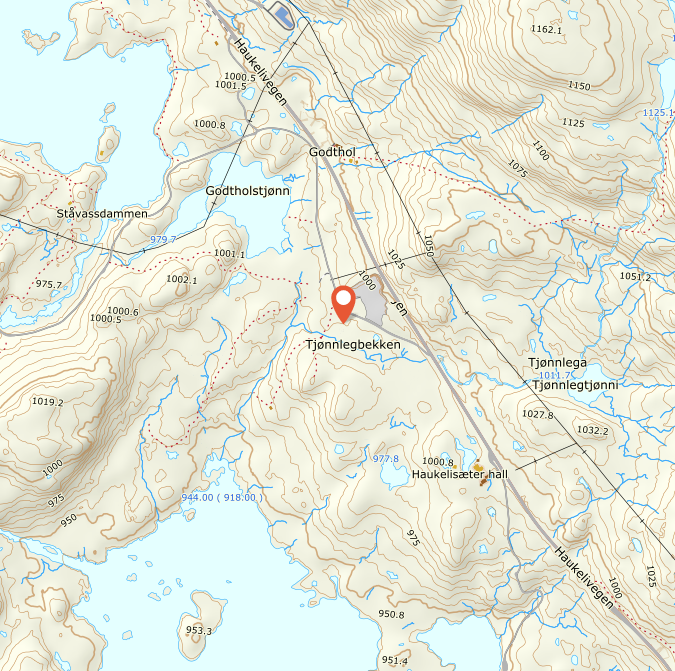
\includegraphics[width=\textwidth]{./fig_Norway/Haukeli_site}
% 		\caption{}\label{fig:site:kartverket}
% 	\end{subfigure}
% 	\caption{Model elevation map of Northern Europe (\protect\subref{fig:site:Norway}) and South Norway (\protect\subref{fig:site:Nzoom}). \subref{fig:site:Norway}  shows the model domain of MEPS.
% Elevation according to the shading. \protect\subref{fig:site:kartverket}: topographical map of the measurement site \citep{geonorge_dtm_2018}.} \label{fig:site}
% \end{figure}
\begin{figure}[!t]
  \begin{tabular}[t]{cc}
    \begin{subfigure}[b]{0.5\columnwidth}
      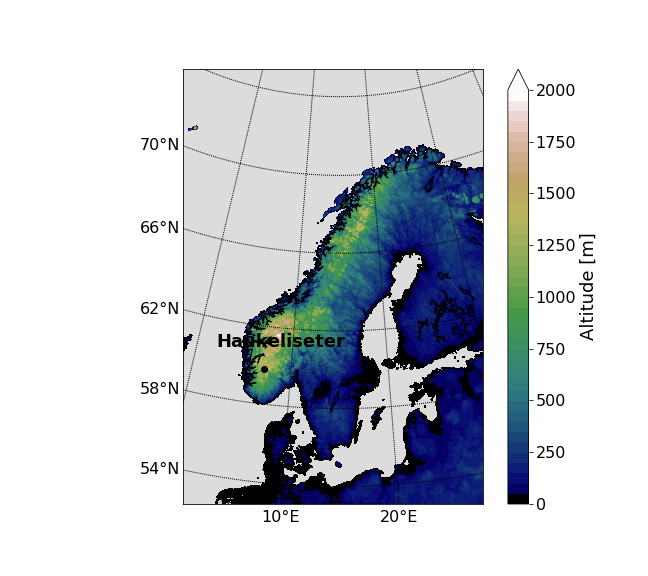
\includegraphics[trim={0cm 0cm 1.6cm 1.cm},clip,width=\textwidth]{./fig_Norway/Norway_elevation_MEPS}
      \caption{}\label{fig:site:Norway}
    \end{subfigure}
    & 
    \begin{tabular}[b]{c}
      \begin{subfigure}[b]{0.5\columnwidth}
        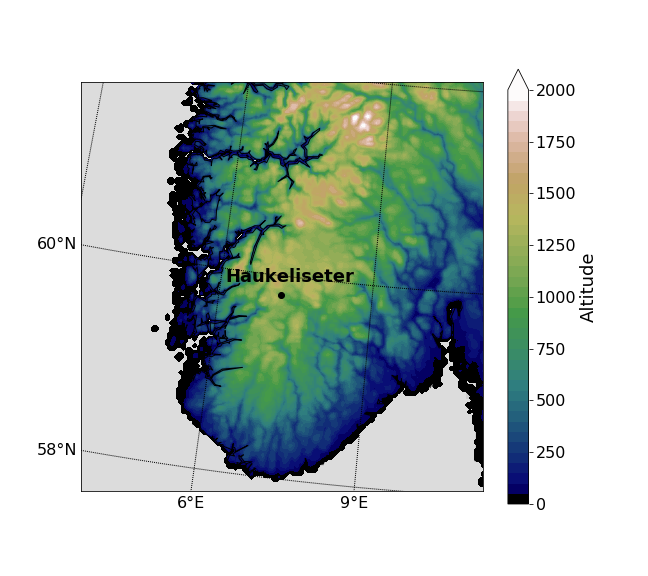
\includegraphics[trim={1.cm 2.2cm 1.8cm 2.4cm},clip,
 		width=\textwidth]{./fig_Norway/South_Norway_MEPS}
        \caption{}\label{fig:site:Nzoom}
      \end{subfigure}\\
      \begin{subfigure}[b]{0.52\columnwidth}
        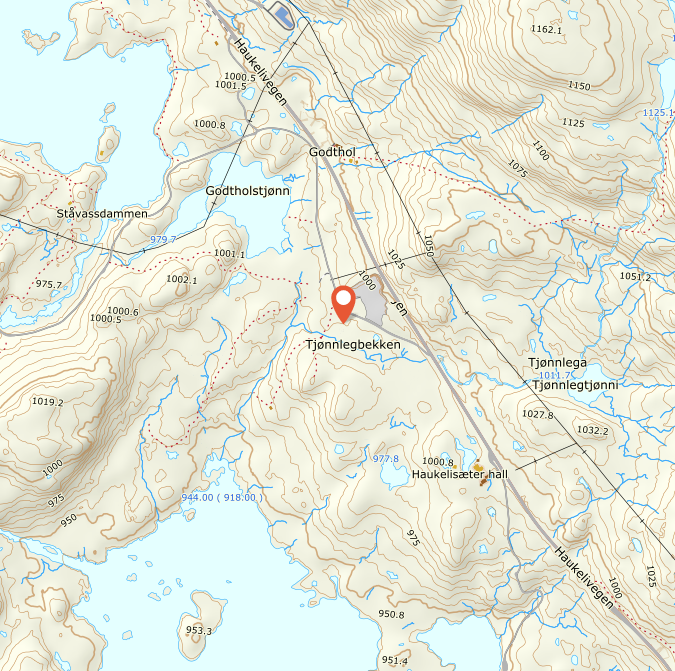
\includegraphics[trim={.3cm 2.2cm 1.8cm 2.4cm},clip,width=\textwidth]{./fig_Norway/Haukeli_site}
        \caption{}\label{fig:site:kartverket}
      \end{subfigure}
    \end{tabular}
  \end{tabular}
  \caption{Model elevation map of Northern Europe (\protect\subref{fig:site:Norway}) and Southern Norway (\protect\subref{fig:site:Nzoom}), where the model domain of MEPS are presented in Lambert projection. The elevation corresponds to the legend of \protect\subref{fig:site:Nzoom}. A topographic map of the measurement site is shown in \protect\subref{fig:site:kartverket} \citep{kartverket_norgeskart_2018}.} \label{fig:site}
\end{figure}